\chapter{Introduction}
What and where is dark matter? For a question so central to cosmology and particle physics, the prospects for finding an answer do not at first glance seem promising. As with so many things in physics, we should not by all rights be able to answer the question, nature having hidden itself away in the dark recesses of the universe. But dark matter is all around us and we merely need a window through which to view it. In this work, I will discuss strategies for the direct detection of dark matter: how they offer us a window - however murky - into the dark universe; how they are faced with myriad  uncertainties; and how those uncertainties can be overcome to help us to understand more about what dark matter is and how it is distributed in our tiny patch of the universe.

The question `\textit{What is dark matter?}' is perhaps best answered by reviewing the current evidence for its existence. Evidence for dark matter is found on scales from the Milky Way up to the cosmological horizon, with a range of observations which cannot be adequately explained with the observed constituents of the universe. Dark matter is an invisible component introduced to reconcile these observations with the known laws of physics - most importantly, General Relativity. Beyond this general definition, there are a wide range of particle physics candidates which may play the role of dark matter. These typically derive from theories of physics beyond the Standard Model, meaning that the study of the properties of dark matter can shed light on theories of high energy physics. Many of these proposed dark matter candidates have weak but non-zero interactions with particles of the Standard Model, leading to several avenues through which it is hoped the non-gravitational detection of dark matter may soon be achieved.

In this chapter, we summarise the evidence in support of the dark matter paradigm, including constraints from precision cosmology. We then describe some of the broad classes into which particle dark matter candidates can be categorised, as well as describing a few specific candidates in more detail. Finally, we discuss current progress and constraints from direct and indirect searches for particle dark matter.

\section{Evidence for dark matter}

Dark matter is a key component of the \LCDM paradigm of modern cosmology. In this framework, the energy density of the universe today is dominated by the constant and uniform contribution of the vacuum, $\Lambda$, also referred to as Dark Energy. This contribution exerts a negative pressure and drives the accelerating expansion of the universe which was the subject of the 2011 Nobel Prize in Physics \cite{Riess:1998, Perlmutter:1999}. However, the formation of structure in the early universe is driven by the clustering of an inert, slow moving and as yet undetected matter component \cite{Kolb:1990}: Cold Dark Matter. In \LCDM cosmology, baryonic matter makes up a much smaller fraction of the energy density of the universe. Cosmological experiments allow us to precisely determine the contributions of these various components (see e.\ g.\  WMAP \cite{Hinshaw:2013}, BOOMERanG \cite{MacTavish:2005}, BOSS \cite{Dawson:2013}, BICEP2 \cite{Ade:2014} and CFHTLenS \cite{Kitching:2014} to name just a few.)

A particularly sensitive probe for determining the dark matter contribution to the energy budget of the universe is the measurement of the temperature anisotropies of Cosmic Microwave Background (CMB) photons. These contain an imprint of the acoustic oscillations of the baryon-photon fluid during the era of recombination. The scale of these oscillations is sensitive to the size of the gravitational potential generated in the early universe by dark matter. \note{This is shite and needs fixing, am I talking about BAOs or what?} The recent Planck experiment \cite{PlanckI:2013} measured the angular power spectrum of these CMB temperature anisotropies. Figure~\ref{fig:intro:CMB} shows the results of these measurements, as well as the best fit 6-parameter \LCDM model. The contribution of the cosmological constant, the total matter component, and the separate baryonic and dark matter components to the total energy density of the universe is shown in Table~\ref{tab:intro:Planck}, constrained with an accuracy of less than 3\%. We are lead to the conclusion that $\sim$84\% of the matter content of the universe is in fact dark.

\todo{Also important that we need CDM to form structures see Kolb:1990 - however, this could fold in nicely with N-body stuff...}

\begin{figure}[h]
  \label{fig:intro:CMB}
  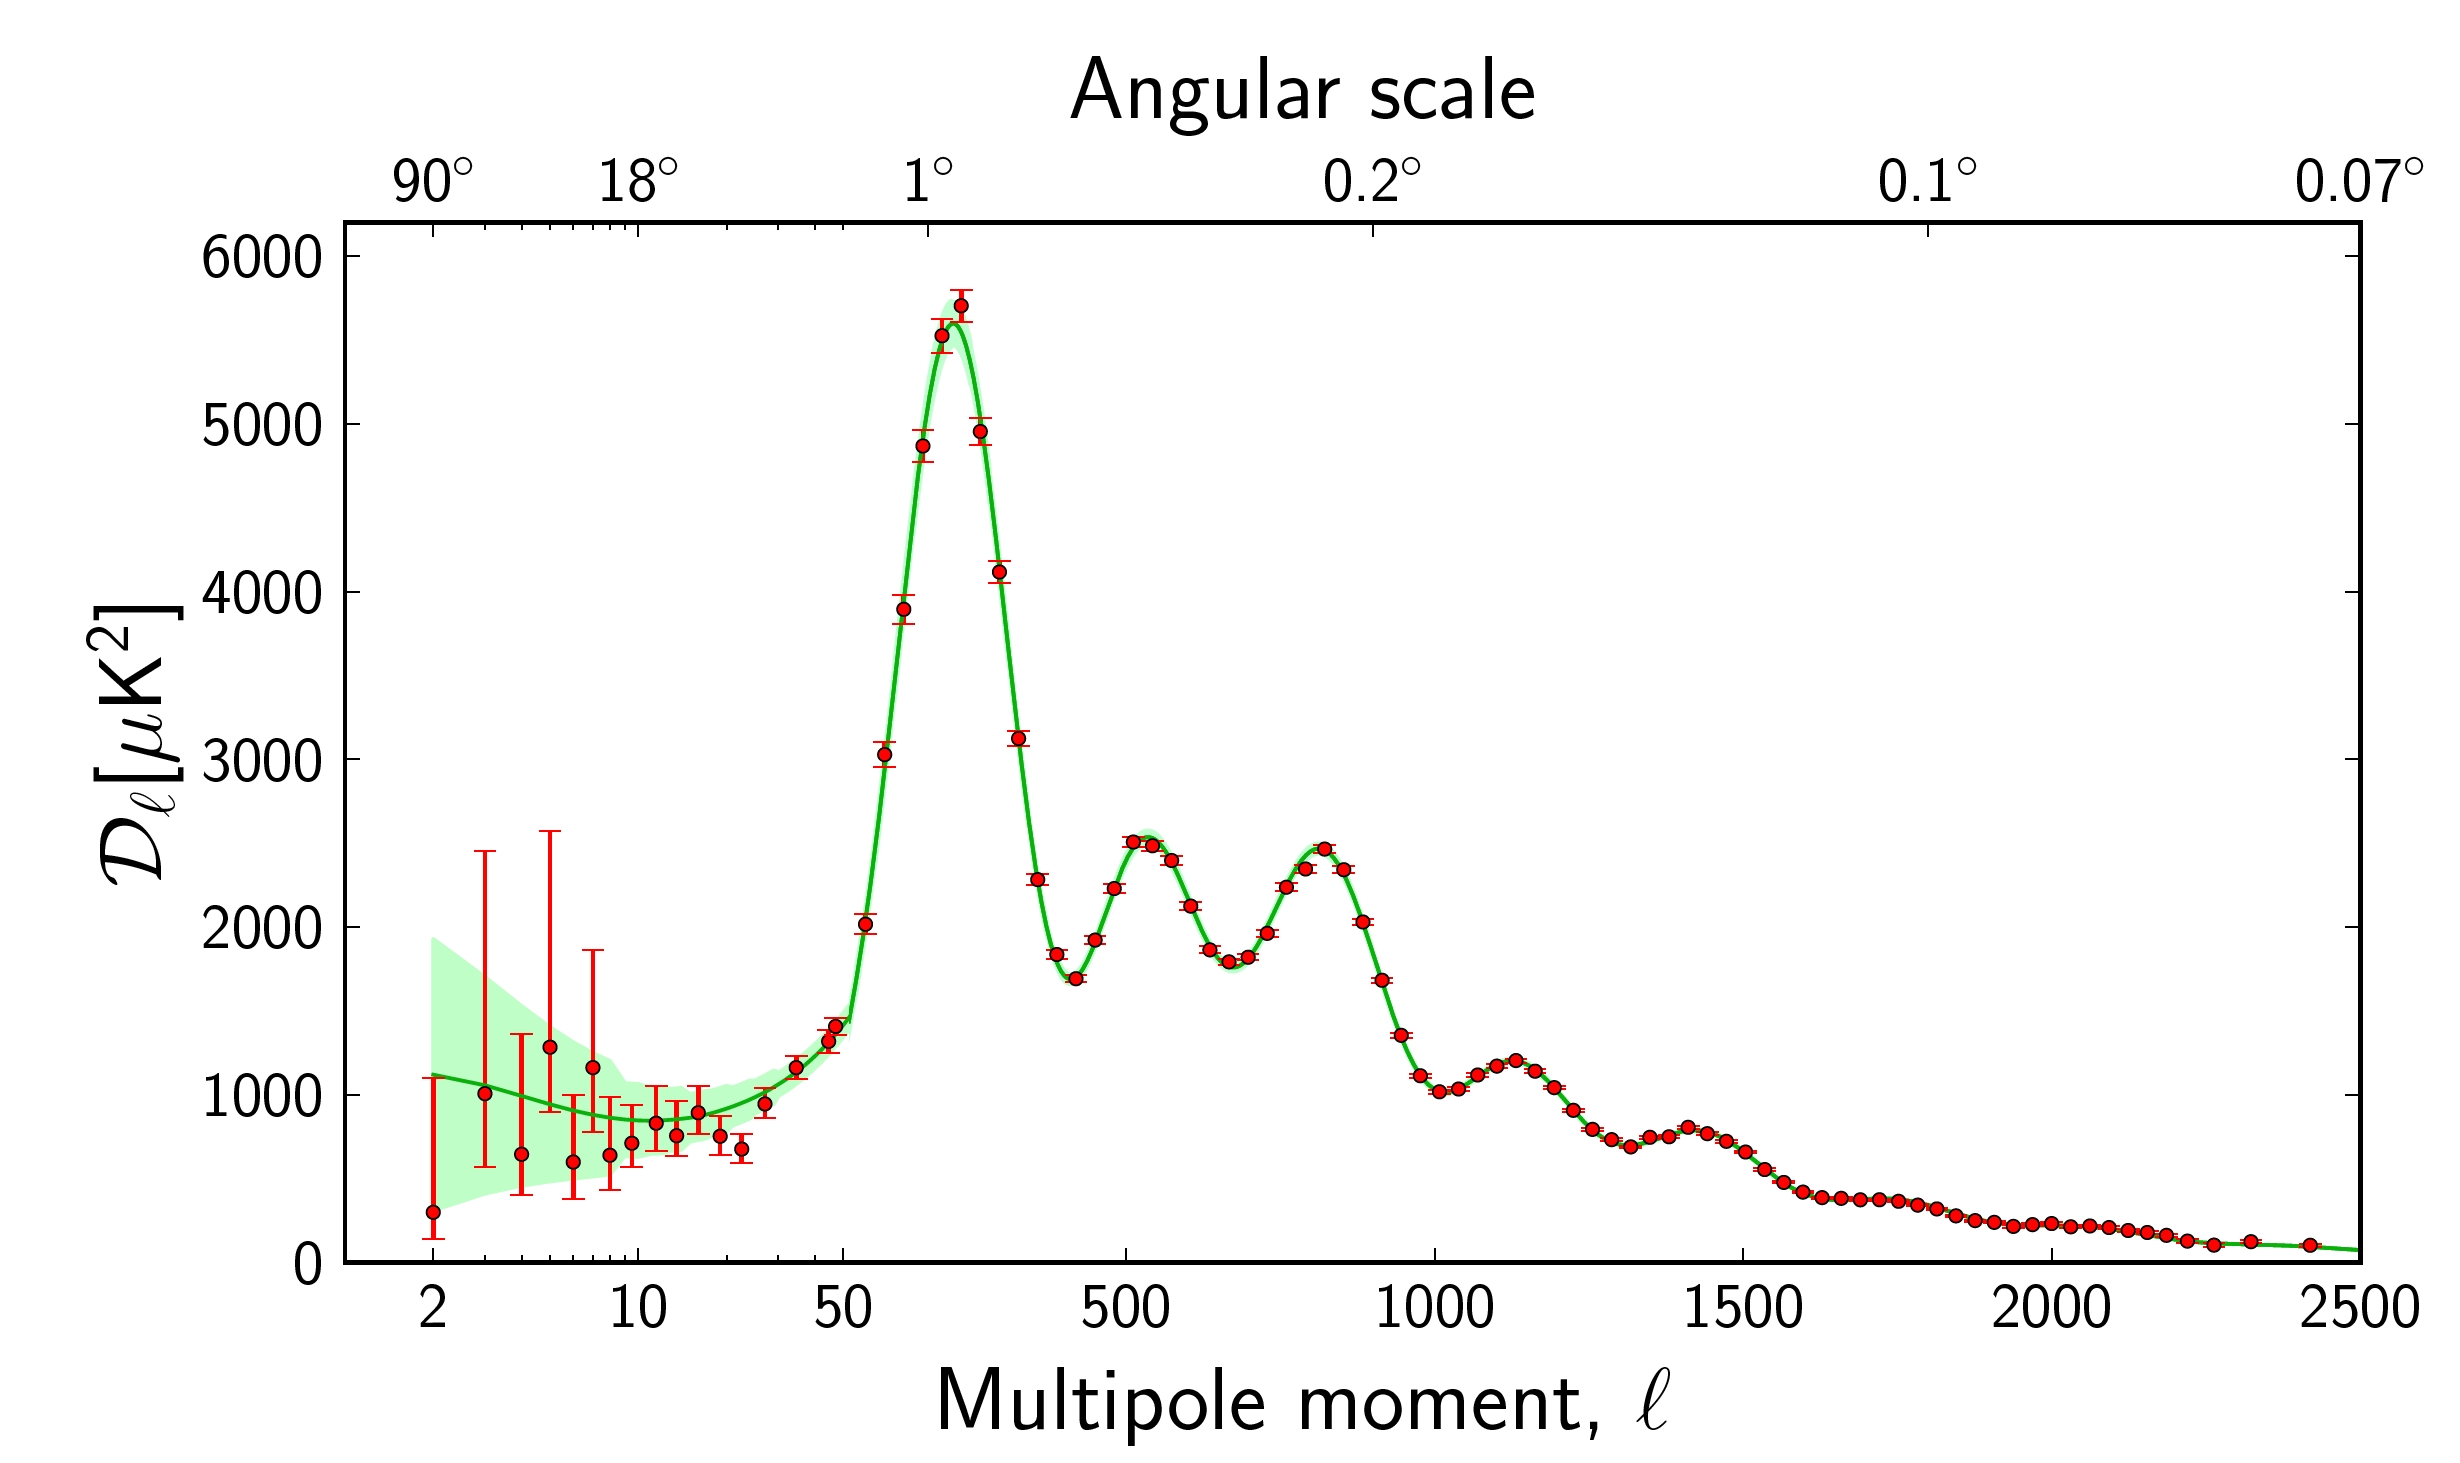
\includegraphics[width=\textwidth]{CMBanisotropies.jpg}
  \caption[CMB anisotropies measured by the Planck experiment]{CMB anisotropies. \note{Need actual caption}}
\end{figure}


\begin{table}
  \begin{center}
	\begin{tabular}{cc}
        \hline\hline
        Parameter & 68\% limits \\
        \hline
        $\Omega_\Lambda$ & 0.686 $\pm$ 0.020 \\
        $\Omega_m h^2$ & 0.1423 $\pm$ 0.0029 \\
        $\Omega_b h^2$ & 0.02207 $\pm$ 0.00033 \\
        $\Omega_c h^2$ & 0.1196 $\pm$ 0.0031 \\
        \hline\hline
	\end{tabular}
  \end{center}
  \caption[Cosmological parameters obtained by the Planck Collaboration]{Energy density of the cosmological constant ($\Lambda$), total matter ($m$), and separate baryonic ($b$) and cold dark matter ($c$) components in units of the critical density \note{define...}, as obtained by the Planck Collaboration \cite{PlanckXVI:2013}. The Hubble parameter is defined as $H_0 = 100 \,\,h \, \textrm{km s}^{-1} \textrm{Mpc}^{-1}$.}
  \label{tab:intro:Planck}
\end{table}

However, the evidence for dark matter is not purely cosmological. In 1933, Zwicky measured the velocity dispersion of galaxies in the Coma cluster \cite{Zwicky:1933}. An application of the Virial Theorem indicated a gravitational mass in the cluster which was several hundred times bigger than that expected from the luminosity of the member galaxies. It is now known that some of this mass is in the form of hot ($\sim$1 million K), X-ray emitting intracluster gas \cite{Sanders:2013}. Nonetheless, a discrepancy remains; current estimates of the mass-to-light ratio of the Coma cluster give a value of roughly 150 times that of the Sun \cite{Fusco-Femiano:1994,Makino:1994}. However, the Coma cluster does not appear to be unusual. Measurements of the masses of a large number of galaxy clusters using gravitational lensing \cite{Okabe:2013}, X-ray observations \cite{Ettori:2013} and dynamical estimates \cite{Carlberg:1995} indicate that a significant fraction of a cluster's mass must be dark.

\todo{Galactic scales - local estimates}
\todo{Talk about dynamical, lensing and X-ray masses?}
\todo{Need to talk about lensing observations...}
\todo{Nonbaryonic nature determined by primordial nucleosynthesis...}
\todo{Cite Lyndzo!}
\todo{Lensing?}
\todo{N-body}


\note{How long should the intro be - timings and planning? DMO8}
\note{Start paper...}



\section{Particle dark matter candidates}

Beyond its gravitational contribution to the universe, we appear to know little about the nature of particle dark matter. However, the success of modern cosmology and the lack of a confirmed detection so far means that we do have a grasp on some of the properties of any potential candidate. Taoso \etal \cite{Taoso:2008} present a `10-point test' which must be passed by any particle before it can be considered as a viable dark matter candidate. Here, I will briefly discuss three of these points, namely, that the DM candidate must be cold, neutral and produced with the appropriate relic density.

\note{Discuss those three conditions - coldness, neutrality and relic density; what about being baryonic}

The final condition appearing in the `10-point test' of Taoso \etal asks the question `Can it be probed experimentally?' While there are viable DM candidates which interact only gravitationally (such as the gravitino \note{need a ref}), a wide variety of proposed candidates can interact (however weakly) with the particles of the standard model. While the experimental accessibility of a given DM candidate is not a strict necessity, it allows models to be tested (and either falsified or confirmed) beyond the hypothesis stage. In the next section, we explore the different avenues by which models of particle dark matter may be probed.

\section{Detection of dark matter}

\note{Often justified that if it was created in the early universe it should interact with crossing diagrams}